\documentclass[12pt,letterpaper,final]{report}
\usepackage[utf8]{inputenc}
\usepackage{amsmath}
\usepackage{amsfonts}
\usepackage{amssymb}
\usepackage{amsthm}
\renewcommand\qedsymbol{$\blacksquare$}
\usepackage{enumerate}
\usepackage{hyperref}
\usepackage{pdfpages}
\usepackage{graphics}
\usepackage{graphicx}
\usepackage{tikz}
\usepackage{tikz-qtree}
\usetikzlibrary{automata,arrows}
\usepackage[
  backend=biber,
  style=authoryear,
  sorting=nyt          % sort by name, year, title
]{biblatex}
\addbibresource{references.bib}

\author{Marius Zimand}
\author{Jonathan Llovet}

\begin{document}

\fbox{
  \vbox{
    \begin{flushleft}
      Jonathan Llovet \\  % authors' names
      COSC 417 \\  %class
      2026-02-12, 11:59 PM (EST) \\  % date
    \end{flushleft}
    \center{\Large{\textbf{Assignment 1}}}
    %\end{mdframed}
  } % end vbox
} % end fbox
\vline

{\bf Problem 1.} Let $A = \{x,y\}$ and $B= \{x,y,z\}$.
\begin{enumerate}
  \item  Is $A$ a subset of $B$?

        Yes

  \item  Is $B$ a subset of $A$?

        No

  \item What is $A \cup B$?

        $\{x,y,z\}$

  \item  What is $A \cap B$?

        $\{x,y\}$

  \item  What is $A \times B$?

        $\{(x,x), (x,y), (x,z), (y,x), (y,y), (y,z)\}$

  \item  What is ${\cal P}(B)$? (${\cal P}(B)$ is the powerset of $B$).

        $\{
          \emptyset,
          \{x\},
          \{y\},
          \{z\},
          \{x,y\},
          \{x,z\},
          \{y,z\},
          \{x,y,z\}
          \}$

  \item What is ${\cal P}({\cal P}(A))$?

        Recall that
        \[
          \begin{array}{lll}
            A           & = \{x,y\}                              \\
            {\cal P}(A) & = \{\emptyset, \{x\}, \{y\}, \{x,y\}\} \\                                                                                                                                     \\ % quadruple
          \end{array}
        \]

        Arranging the elements by their cardinality,

        \[
          {\cal P}({\cal P}(A)) = A_0 \cup A_1 \cup A_2 \cup A_3 \cup A_4
        \]

        where

        \[
          \begin{array}{lll}
             & A_0 = \emptyset                                                                                                                                                                       \\\\ % empty set
             & A_1 = \{\emptyset\}, \{x\}, \{y\}, \{x, y\}                                                                                                                                           \\\\ % singletons
             & A_2 = \Big\{\emptyset, \{x\}\Big\}, \Big\{\emptyset, \{y\}\Big\}, \Big\{\emptyset, \{x, y\}\Big\}, \Big\{\{x\}, \{y\}\Big\}, \Big\{\{x\}, \{x, y\}\Big\}, \Big\{\{y\}, \{x, y\}\Big\} \\\\ % pairs
             & A_3 = \Big\{\emptyset, \{x\}, \{y\}\Big\}, \Big\{\emptyset, \{x\}, \{x, y\}\Big\}, \Big\{\emptyset, \{y\}, \{x, y\}\Big\}, \Big\{\{x\}, \{y\}, \{x, y\}\Big\}                         \\\\ % triples
             & A_4 = {\cal P}(A) = \Big\{\emptyset, \{x\}, \{y\}, \{x, y\}\Big\}
          \end{array}
        \]

  \item What is the size of ${\cal P}(A) \times {\cal P}(B)$?


        The cardinality of a power set $X$ is $2^{\vert X \vert}$.

        $A = \{x,y\}$ and $B= \{x,y,z\}$. Their cardinalities are $\vert A \vert = 2$, $\vert B \vert = 3$.

        Hence, the size of ${\cal P}(A)$ is $2^2 = 4$, and the size of ${\cal P}(B)$ is $2^3 = 8$.

        Therefore the size of ${\cal P}(A) \times {\cal P}(B)$ is $2^{\vert A \vert} \times 2^{\vert B \vert}$, or

        $2^{2} \times 2^{3} = 4 \times 8 = 32$


\end{enumerate}

\pagebreak
{\bf Problem 2.}	Show that the set $A =\{-1, 0\} \cup \mathbb{N}$ is a countable infinite set by giving an explicit bijective function $f : {\mathbb N} \rightarrow A$.  Prove that your function $f$ is a bijection, by showing that it is 1-to-1 (no two natural numbers map to the same element) and onto (every element in $A$ is the image of some natural number).
\medskip

Let $f(n) = n - 2$.
First, we will write $A =\{-1, 0\} \cup \mathbb{N}$ as one set:

\[
  \begin{aligned}
    \mathbb{N} & = \{1,2,3,4,5,\ldots\}  \\
    A          & = \{-1,0,1,2,3,\ldots\}
  \end{aligned}
\]

By applying $f$ to each of the elements of $\mathbb{N}$ in turn, we will obtain:

\[
  \begin{aligned}
    f(\mathbb{N}) & = \{f(1), f(2), f(3), f(4), f(5), \ldots\} \\
                  & = \{-1,0,1,2,3,\ldots\}                    \\
                  & = A
  \end{aligned}
\]
We will prove that $f(n)$ is a bijection in two parts.
In the first part, we will show by contraposition that $f$ is injective, and in the second part we will show by induction that $f$ is surjective.

\medskip
{\bf Part 1: Injective (1-1)}: No two natural numbers map to the same element.

We wish to show that $f: \mathbb{N} \to A$ is injective, i.e.
\begin{equation}
  \forall a, b \in \mathbb{N}, a \ne b \implies f(a) \ne f(b) \label{eq:1}
\end{equation}

We will prove this by contraposition. The contrapositive of the preceding statement is
\begin{equation}
  \forall a, b \in \mathbb{N}, f(a) = f(b) \implies a = b \label{eq:2}
\end{equation}

This is what we will tackle to prove the original. Let
\[
  \begin{aligned}
    a & = c \\
    b & = d
  \end{aligned}
  \quad \text{where } c, d \in \mathbb{N}.
\]

Then
\[
  \begin{aligned}
     &            & f(c)  & = f(d)  &  & \text{using particular values for a, b} \\
     &            & c - 2 & = d - 2 &  & \text{by substitution for $f(n)$}       \\
     & \therefore & c     & = d     &  & \text{by adding 2 to both sides}
  \end{aligned}
\]

From preceding, we conclude \eqref{eq:2}. But therefore, because contrapositives are logically equivalent, we conclude that \eqref{eq:1} is true, viz. $\forall a, b \in \mathbb{N}, a \ne b \implies f(a) \ne f(b)$, and that the function $f$ is injective.

\medskip
{\bf Part 2: Surjective (Onto)}: Every element in A is the image of some natural number.

We wish to show that $f: \mathbb{N} \to A$ is surjective, i.e.
\begin{equation}
  \forall a \in A, \exists n \in \mathbb{N}: a = f(n) \label{eq:3}
\end{equation}

We will prove this by induction.

\medskip
{\bf Basis step: $P(A_0)$}
\medskip

We wish to show:
\begin{equation}
  \exists n \in \mathbb{N} : f(n) = A_0  \label{eq:4}
\end{equation}

Note that $A_0 = - 1$. Examining this and solving for $n$:

\[
  \begin{aligned}
    f(n)  & = -1 &  &                                \\
    n - 2 & = -1 &  & \text{by definition of $f(n)$} \\
    n     & = 1  &  & \text{by algebra}              \\
  \end{aligned}
\]

But $1 \in \mathbb{N}$. Therefore, \eqref{eq:4} holds.

\medskip
{\bf Induction step: $P(a,k) \implies P(a+1, k+1)$}
\medskip

Assume for some $a \in A$, some $k \in \mathbb{N}$ where $k \ge 1$ that
\[
  P(a,k): a = f(k)
\]

Or, more usefully, substituting for $f(k)$,

\begin{equation}
  P(a,k): a = k - 2 \tag{Inductive Hypothesis} \label{eq:5}
\end{equation}
\medskip

We wish to show that $P(a,k) \implies P(a+1, k+1)$. Consider:

\begin{align*}
  a     & = k - 2     &  & \text{By $\eqref{eq:5}$}           \\
  a + 1 & = k + 1 - 2 &  & \text{By adding $1$ to both sides} \\
  a + 1 & = f(k+1)    &  & \text{By definition of $f(k+1)$}
\end{align*}

This is what we wished to derive, since $P(a+1, k+1): a + 1 = f(k+1)$. But therefore, $P(a,k) \implies P(a+1, k+1)$ holds. Hence, we conclude by the principle of mathematical induction that \eqref{eq:3} holds. That is, we conclude that $\forall a \in A, \exists n \in \mathbb{N}: a = f(n)$, or to put it simply, that the function $f$ is surjective.

\medskip
{\bf Conclusion: $f$ is bijective, $A$ is countably infinite}
\medskip

Therefore, having shown that the function $f(n)$ is injective and surjective, we conclude that it is bijective. But therefore, by definition of a countable infinite set, we conclude further that $A =\{-1, 0\} \cup \mathbb{N}$ is a countably infinite set, since we have found a bijective function $f: \mathbb{N} \to A$.

\qed



\pagebreak
{\bf Problem 3.} For each of the following languages, give the state diagram of a DFA with the specified number of states that recognizes the language. The alphabet is $\Sigma = \{0,1\}$.

\begin{enumerate}

  \item $\{w \colon \mbox{ $w$ contains at least one $0$ and one $1$}\}$, with $4$ states.

        \medskip

        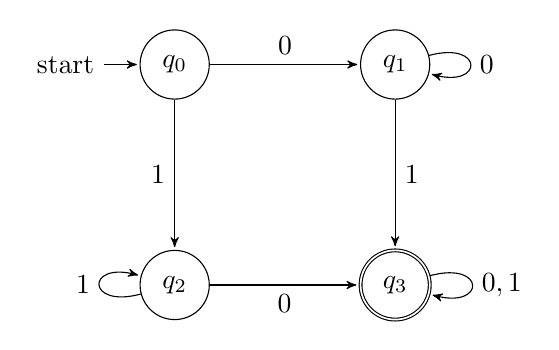
\begin{tikzpicture}[>=stealth',shorten >=1pt,auto,node distance=2.8cm]

          \node[initial, state] (0) {$q_{0}$};
          \node[state] (1) [right of=0] {$q_{1}$};
          \node[state] (2) [below of=0] {$q_{2}$};
          \node[state, accepting] (3) [below of=1] {$q_{3}$};

          \path[->]
          (0) edge node[above] {$0$} (1)
          (0) edge node[left] {$1$} (2)

          (1) edge node[right] {$1$} (3)
          (1) edge [loop right] node {$0$} (1)

          (2) edge [loop left] node {$1$} (2)
          (2) edge node[below] {$0$} (3)

          (3) edge [loop right] node {$0,1$} (3)
          ;
        \end{tikzpicture}

  \item $\{w \colon \mbox{ $w$ has $0$ in every odd position}\}$, with $3$ states.

        \medskip

        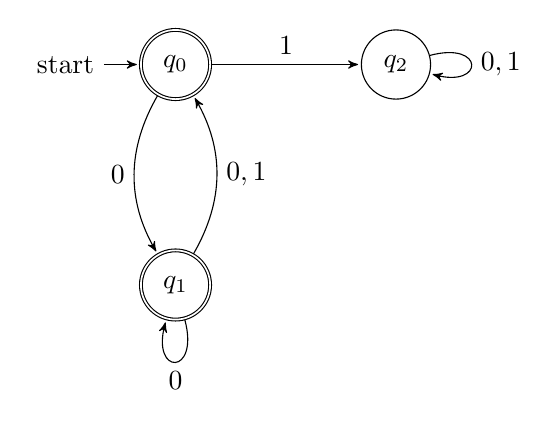
\begin{tikzpicture}[>=stealth',shorten >=1pt,auto,node distance=2.8cm]

          \node[initial, state, accepting] (0) {$q_{0}$};
          \node[state, accepting] (1) [below of=0] {$q_{1}$};
          \node[state] (2) [right of=0] {$q_{2}$};

          \path[->]
          (0) edge [bend right] node[left] {$0$} (1)
          (0) edge node[above] {$1$} (2)

          (1) edge [bend right] node[right] {$0,1$} (0)
          (1) edge [loop below] node {$0$} (1)

          (2) edge [loop right] node {$0,1$} (2)
          ;
        \end{tikzpicture}

\end{enumerate}

\pagebreak
{\bf Problem 4.}  Recall that an infinite  set $A$ is countable if there is a \emph{bijective}  function $f: {\mathbb N} \rightarrow A$.  Show that if there is an \emph{onto} function
$g: {\mathbb N} \rightarrow A$, then $A$ is countable. In other words, you need to show how you can modify $g$ to obtain a bijective function $f$ that enumerates $A$.

There are two cases to consider here: 1. when the \emph{onto} function is already \emph{one-to-one} and 2. when the \emph{onto} function is not already \emph{one-to-one}.

In case 1, because the function is both \emph{onto} (surjective) and \emph{one-to-one} (injective), the function is already bijective by definition of bijective, and there is nothing we need to do to the function.

In case 2, the function $f$ is \emph{onto} (surjective), but it is not \emph{one-to-one} (injective). This means that $f: \mathbb{N} \to A$ covers every element of A, but there are collisions where for $a, b \in \mathbb{N}, f(a) = f(b) \wedge a \ne b$.

We are going to take a similar approach to \textcite[p.204]{sipser2013} when he is showing an enumeration of the rational numbers. There, he defines a procedure for iterating through pairs of natural numbers in a matrix to produce an enumeration that is both surjective and injective. In the case of the enumeration of the rationals $f: \mathbb{N} \to \mathbb{Q}$, his procedure generates an intermediate sequence of numbers that are a multiset of the rationals, with some numbers appearing multiple times, because they are generated mechanically according to the procedure but are actually equivalent to numbers that have already appeared in the sequence.

\includegraphics[width=0.8\linewidth]{sipser-rationals-table.png}

Take for example $2/2$, the fifth number to appear in the sequence. When it is reduced to simplest form, $2/2 = 1/1$, which has already appeared in the sequence. In order to satisfy the requirement of a \emph{one-to-one} function and produce the set of rationals, he skips the elements in the sequence such as this one that have already appeared earlier on in the sequence.

Generalizing from Sipser's approach here, we can say that for a function $f: \mathbb{N} \to A$, where A is an infinite set, if $f$ is \emph{onto}, we can modify the function in the following way to make it \emph{one-to-one} as well. If the enumeration produces a collision, skip the element that produces the collision and have $f(n)$ be mapped to the next element of the sequence that does not produce a collision. Let $A_{seq}$ represent the intermediate sequence of elements that is used in a construction of the enumeration of set $A$ (analogous to the sequence created by the procedure used by Sipser in the matrix copied above on the way to enumerating $\mathbb{Q}$). If $A_{seq}$ is a sequence of elements, then $n \in \mathbb{N}, f(n) \in A_{seq}$. If $f(n)$ appears in any of the previously mapped elements, then skip elements of $A_{seq}$ until $f(n)$ is a new unique element.

Put a bit more formally, let:
\[
  A_{1 \to n} = \{f(1), f(2), f(3), \ldots, f(n)\}
\]
Then $A_{1 \to n} \subseteq A$ is a subset of $A_{seq}$, and $A_{1 \to n}$ consists of a partial enumeration of $A$. For the element $f(n+1)$, if $f(n+1) \in A_{1 \to n}$, then let $f(n+1)$ be mapped to the least subsequent element $a \in A_{seq}$ such that $a \not\in A_{1 \to n}$.
By performing this modification, we will filter out the collisions, resulting in the function $f: \mathbb{N} \to \mathbb{A}$ being \emph{one-to-one} and consequently bijective.

\qed


\pagebreak
{\bf Problem 5. }
Let $A$ and $B$  be two infinite countable sets.  Show that  $A \cup  B$ is also an infinite countable set. You need to show how to obtain an enumeration of $A \cup B$ if you have an enumeration $A = \{f(1), f(2), \ldots \}$ and an enumeration of $B = \{g(1), g(2), \ldots \}$ (in other words you need to explain how you can list one-by-one all the elements in $A \cup B$.)

To demonstrate how we can construct an enumeration, first it is helpful to consider the approach taken by \textcite[p.204]{sipser2013} when demonstrating that there is a bijection $f: \mathbb{N} \to \mathbb{Q}$ that enumerates the rationals.

\includegraphics[width=0.8\linewidth]{sipser-rationals-table.png}

There he builds an enumeration by weaving through arrangements of the natural numbers, such that the numerator is determined by the row, the denominator is determined by the column. We proceed in the diagonalized pattern that is shown in the diagram, skipping any of the numbers that reduce to a value we have already seen. Notably, we do not try to run through all of the elements of the first row before moving on to the second row, since we would never finish the first row by this method.

Similarly, we do not want to try to run through all of the elements of $A$ in our enumeration before introducing elements of $B$. Rather, we should interleave the sets as follows to enumerate the elements of $A \cup B$:

\[
  \{f(1),g(1),g(2),f(2),f(3),g(3),g(4),f(4),\ldots\}
\]

Consider the following diagram.

\begin{center}
  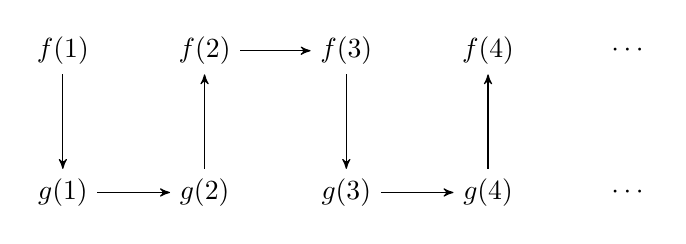
\begin{tikzpicture}[>=stealth', node distance=1.8cm]
    % top row: f
    \node               (f1) {$f(1)$};
    \node [right of=f1] (f2) {$f(2)$};
    \node [right of=f2] (f3) {$f(3)$};
    \node [right of=f3] (f4) {$f(4)$};
    \node [right of=f4]      {$\cdots$};

    % bottom row: g
    \node [below of=f1] (g1) {$g(1)$};
    \node [right of=g1] (g2) {$g(2)$};
    \node [right of=g2] (g3) {$g(3)$};
    \node [right of=g3] (g4) {$g(4)$};
    \node [right of=g4]      {$\cdots$};

    % zigzag arrows
    \draw[->] (f1) -- (g1);
    \draw[->] (g1) -- (g2);
    \draw[->] (g2) -- (f2);
    \draw[->] (f2) -- (f3);
    \draw[->] (f3) -- (g3);
    \draw[->] (g3) -- (g4);
    \draw[->] (g4) -- (f4);
  \end{tikzpicture}
\end{center}


This can be expressed explicitly as the following function, which is a bijection $h: \mathbb{N} \to A \cup B$

\[
  h(n) =
  \begin{cases}
    f(\lceil \frac{n}{2} \rceil) & \text{if } (n \bmod 4) \in \{0, 1\} \\
    g(\lceil \frac{n}{2} \rceil) & \text{if } (n \bmod 4) \in \{2, 3\}
  \end{cases}
\]

By creating such a function, we have created an enumeration of the set $A \cup B$. Having done so, we have demonstrated that the union of two infinite countable sets is also an infinite countable set.

\qed

\printbibliography

\end{document}
